\leadauthor{Sanderson}

\title{Taxonium: a web-based tool for exploring large phylogenetic trees}
\shorttitle{Taxonium}

\author[1]{Theo Sanderson \orcidlink{0000-0003-4177-2851}}
\affil[1]{The Francis Crick Institute, UK}

\date{}

\maketitle

\begin{abstract}
The recent COVID-19 pandemic has resulted in a step change in the scale of sequencing data, with more genomes of SARS-CoV-2 being sequenced than any other organism on earth. Previous web-based tools for phylogenetic exploration were not able to scale to this challenge, but we have developed Taxonium, a new web-based tool that uses WebGL to allow the exploration of trees with tens of millions of nodes. Taxonium allows visualisation of mutation-annotated trees, where the genotypes at each internal node are indicated, and also links information from metadata to each node. A server side backend permits rapid loading for widely used datasets, while a client-only mode allows the exploration of niche or sensitive data. Taxonium is an open-source tool which can be applied to any large tree. We provide an application for exploring a public tree of more than 1.5 million SARS-CoV-2 sequences at \url{http://cov2tree.org}, the broader Taxonium tool at \url{http://taxonium.org}, and source code at \url{http://github.com/theosanderson/taxonium}.


\end{abstract}

\begin{keywords}
tree | visualisation | phylogenetics
\end{keywords}

\begin{corrauthor}
theo.sanderson\at crick.ac.uk
\end{corrauthor}

\section*{Introduction}\label{s:introduction}

Genomic researchers responded to the emergence of SARS-CoV-2 with rapid collaboration at unprecedented scale. Open protocols were quickly generated for amplicon sequencing \citep{Tyson2020}, and allowed researchers across the globe to produce an ever-growing genomic datasets stored both in the INSDC \citep{insdc}, and more comprehensively in GISAID \citep{shu2017gisaid}, which has recently surpassed 10 million sequences. Importantly, new tools were also developed to understand the functional diversity of these samples, by assigning them into lineages proposed by the community \citep{rambaut2020dynamic, o2021assignment}, and allowing interactive exploration of trends in these data over time \citep{hodcroft_2021, chen2022cov, outbreakinfo}.

The vast scale of these datasets has posed challenges for the array of tools that researchers had previously relied upon to manipulate, analyse, and visualise genomic data. In particular, the construction of phylogenetic trees, and the visualisation of these trees, has been a bottleneck in the analysis of SARS-CoV-2 genomic data. There are two broad responses possible to this issue. The first is to downsample the sequences analysed in order to create a smaller dataset with which existing tools are able to work efficiently, while maintaining much of the sequence diversity present. This has been an important approach, and has allowed NextStrain \citep{nextstrain} to provide one of the most used and most powerful tools for exploring SARS-CoV-2 genetic diversity. Briefly, the NextStrain pipeline downsamples sequences in a rational way, and then uses iqtree \citep{iqtree} to assemble them into a tree, assigns chronology and ancestral states to this tree using TreeTime \citep{treetime}, and displays the results in a user-friendly interactive interface using Auspice \citep{nextstrain}. All three of these post-downsampling stages are bottlenecks which prevent the use of full datasets, and so NextStrain analyses are typically limited to \textasciitilde~4,000 nodes -- sampled in a structured way to ensure they either provide an overview of the pandemic or hone in on particular sequences of interest.

\begin{figure}
\begin{center}
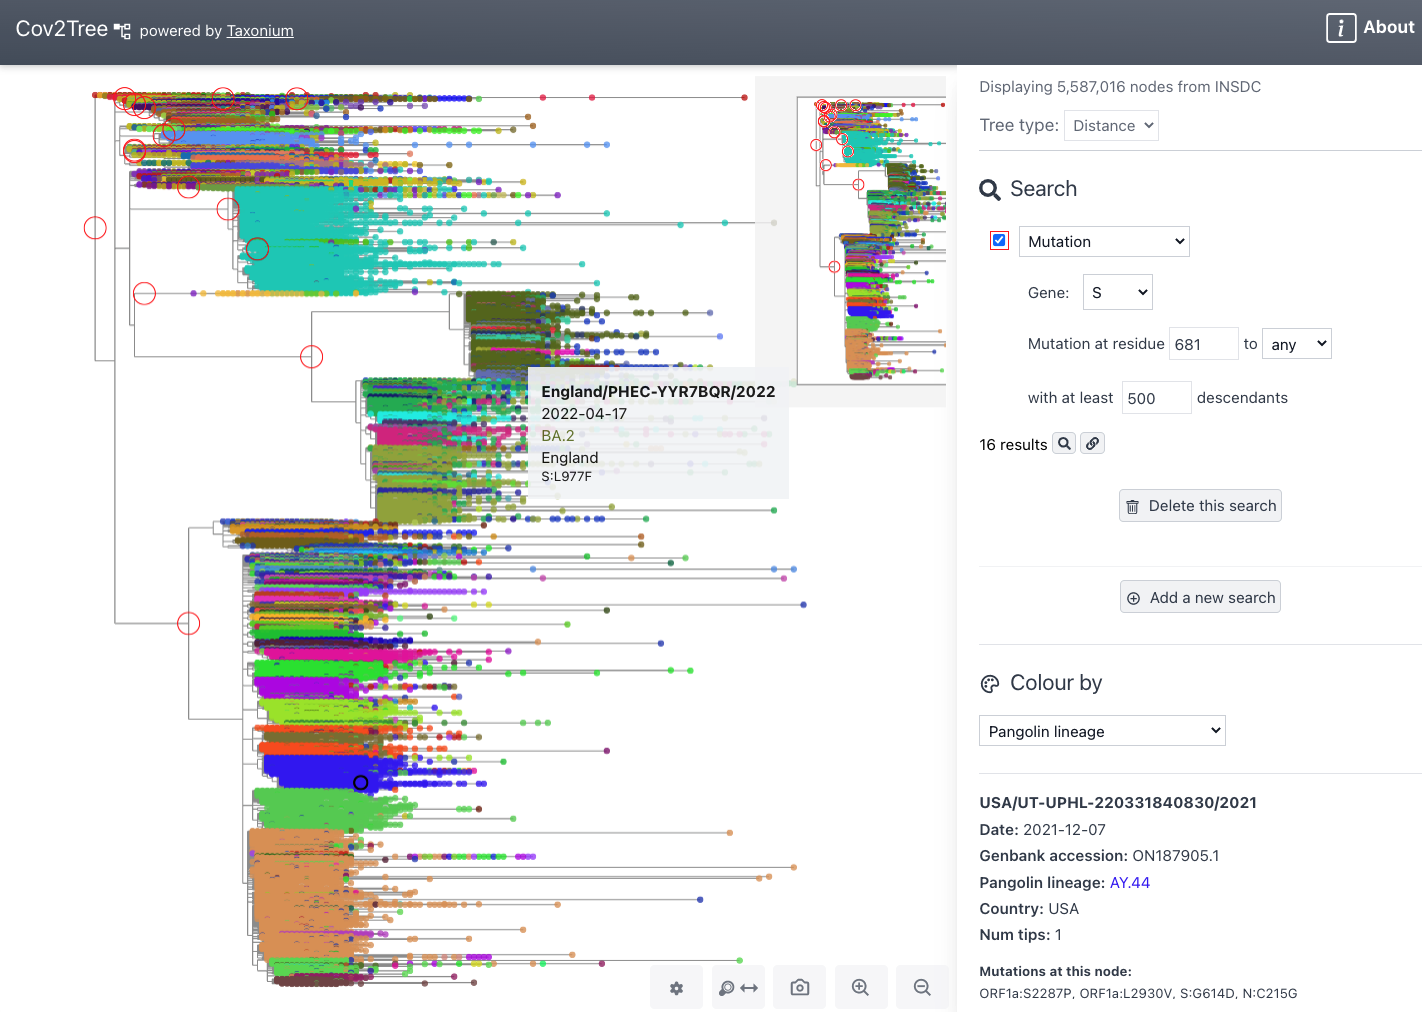
\includegraphics[width=\linewidth]{Figures/screenshot2.png}
\end{center}
\caption{The Taxonium web client displaying a 5,587,016 node tree of SARS-CoV-2 sequences. The left hand panel shows the zoomable tree with a minimap for orientation, and the right hand panel provides options for searching for nodes and for changing the colour scheme. Hovering over a node shows information in a tooltip, while clicking on a node displays further information in the right-hand panel.}
\label{fig:taxonium_client}
\end{figure}

The new scale of data available provides an impetus to develop new tools that are able to work with these large datasets without downsampling. Recently the development of UShER \citep{usher} has permitted larger trees to be built than ever previously. UShER takes a starting tree, built with iqtree or a similar approach, and incrementally adds sequences by maximum parsimony. For densely sampled sequencing efforts, as in the SARS-CoV-2 pandemic, such an approach still yields tree topologies of very high quality. To turn this distance tree into a time tree, by estimating a time associated with each node in the tree, we recently developed Chronumental \citep{chronumental} which uses stochastic gradient descent to efficiently construct chronologies from very large trees, which was not possible with previous approaches. A final necessary component is a tool for exploring these large trees, ideally in a browser.

Here we describe Taxonium, a web-based tool for browsing very large trees. Taxonium scales to trees with millions of nodes, and allows for rapid panning and zooming using WebGL. In addition to reading Newick format trees, Taxonium can also display UShER's mutation-annotated trees which feature mutations at internal nodes. It permits searching for nodes using metadata, and a range of colouring options. Taxonium is available in a server-backed mode, which in a matter of seconds loads to allow exploration of all publicly available SARS-CoV-2 sequences, and also a fully client-side mode, suitable for exploring custom datasets potentially with sensitive data.


\section*{Results}\label{s:results}

\subsection*{The Taxonium Web Client}

The Taxonium web client is a React application that permits the exploration of very large trees. One major bottleneck of previous approaches was the use of web technologies involving SVG or Canvas to visualize the tree. The use of these technologies to explore the a large phylogeny implies the creation of a large DOM tree, which is very expensive in memory and processing. We instead use WebGL, implemented via DeckGL \citep{deckgl}, for efficient visualisation of the tree. Even so, rendering the whole tree would still be too slow, and would involve thousands of nodes overplotted on each pixel when a tree was zoomed out. We address this by rendering a sparsified version of the tree, with the sparsification dependent on the zoom level. This approach allows for a fast and responsive tree exploration.

The input to Taxonium is a tree (e.g. in newick format) and metadata. Metadata is associated with each node of the tree, and the tree can be coloured by any chosen metadata item. Colours are by default calculated using an algorithm that hashes the string of the metadata item, ensuring consistency over time without the need for custom look up tables. In addition, the tree can be searched based on the metadata, with identified nodes circled.

\begin{figure}
\begin{center}
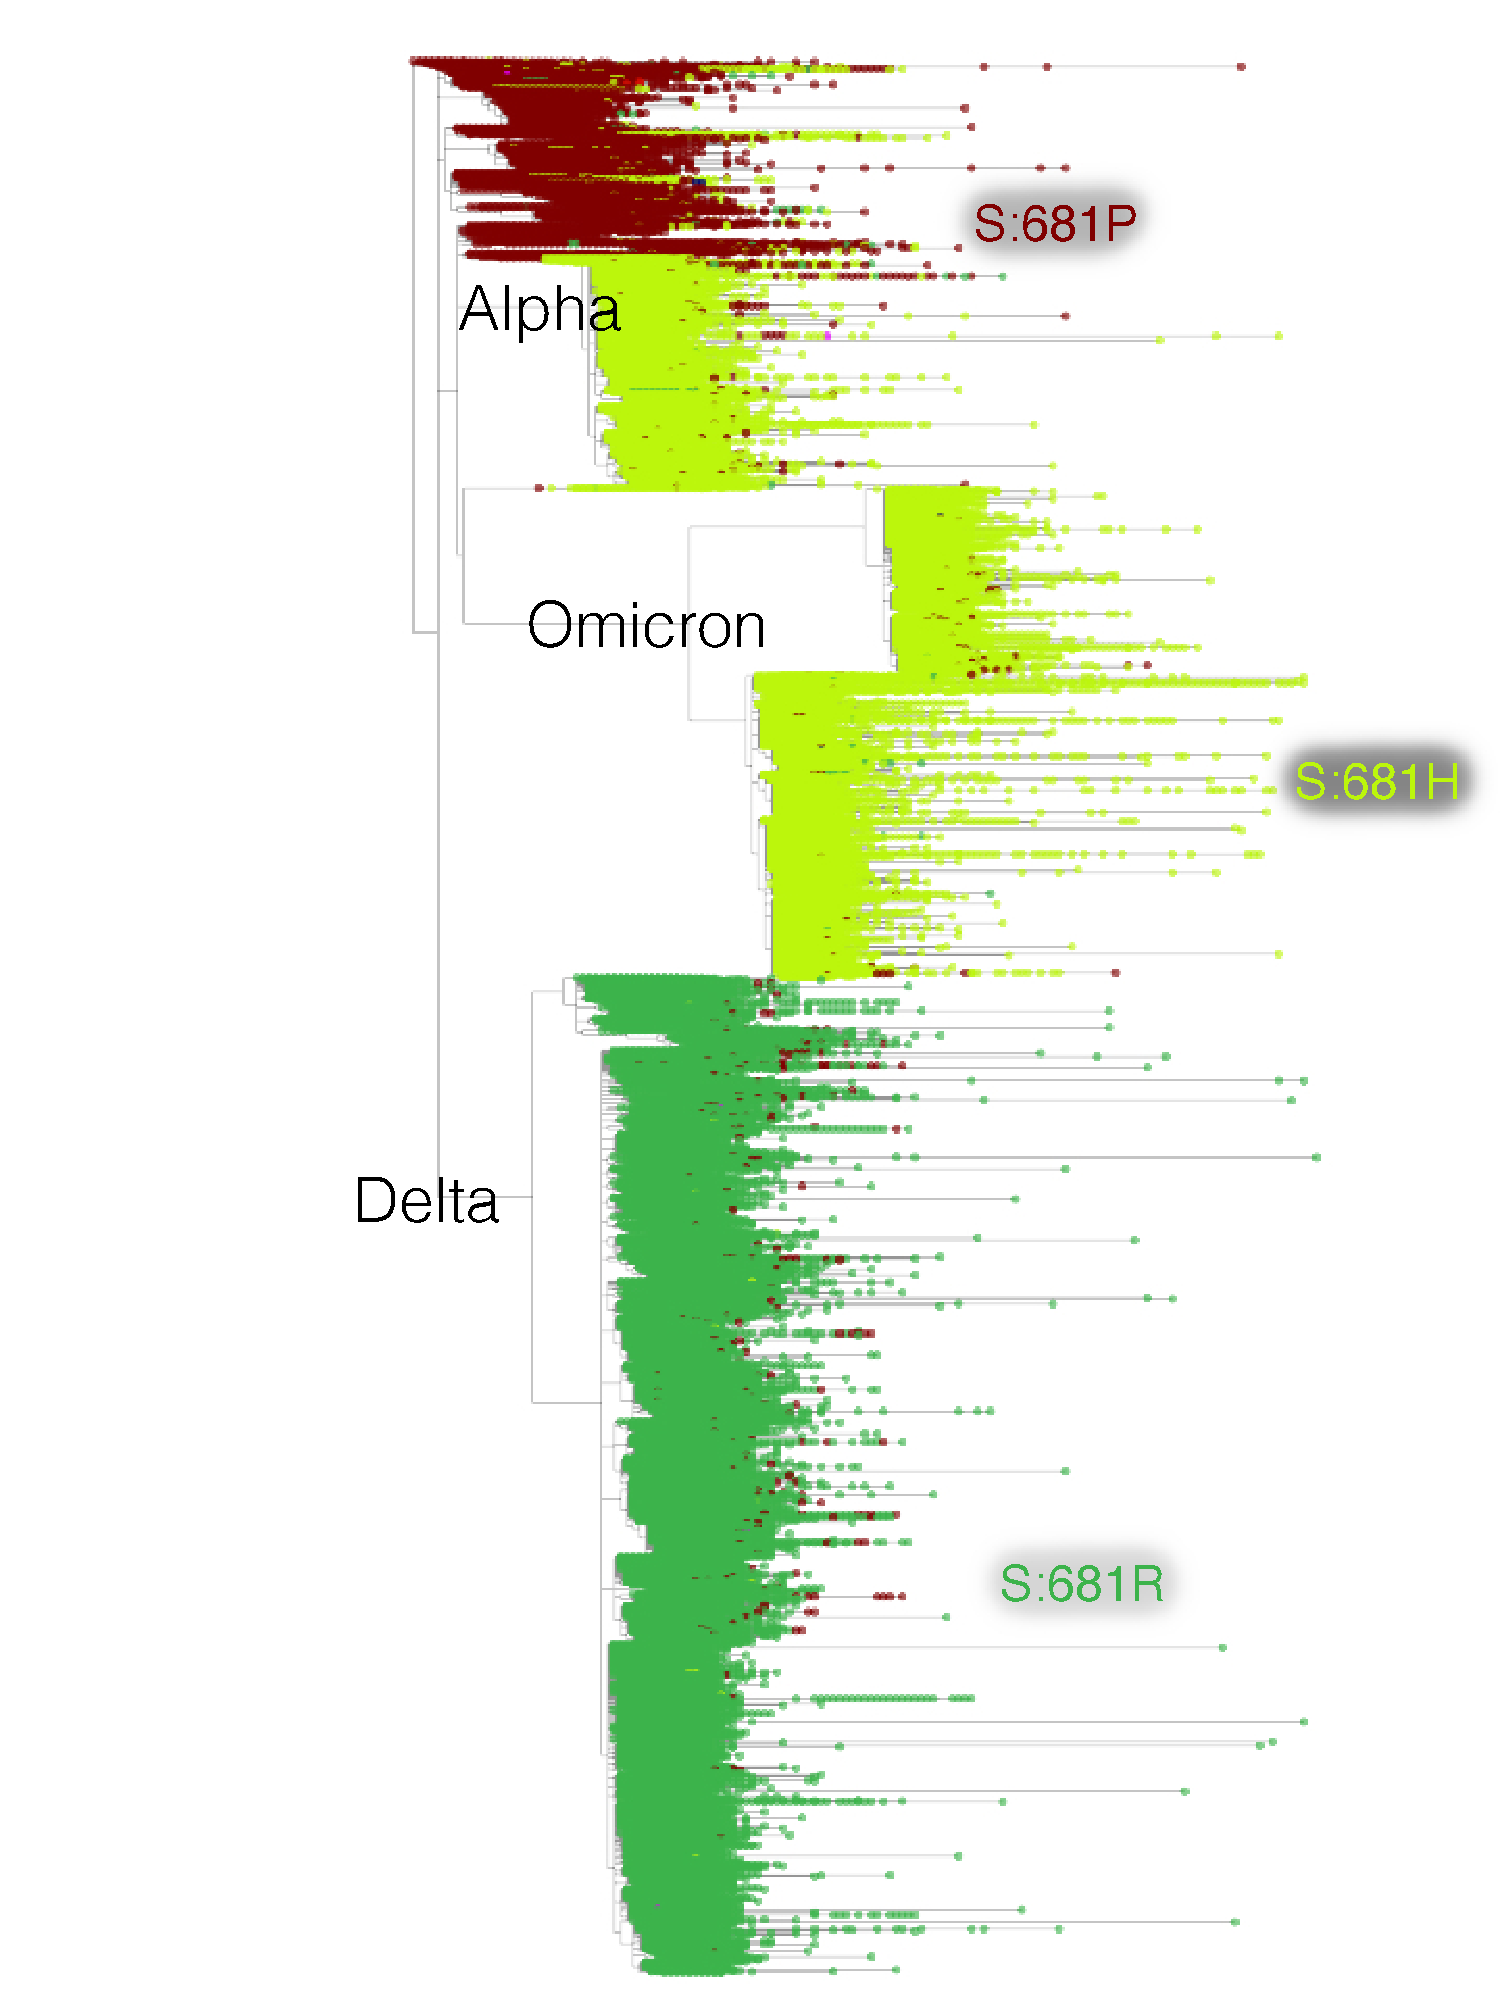
\includegraphics[width=0.9\linewidth]{Figures/681.pdf}
\end{center}
\caption{Overlaying genotype data at position Spike 681 on 4,616,067 SARS-CoV-2 genomes with Taxonium. Taxonium's `Colour by genotype' feature was used to generate this screenshot. Labels have been added here for clarity in this static format.}
\label{fig:681}
\end{figure}

The user interface of the Taxonium web client is shown in Figure 1. The tree, at the left hand side of the screen, can be panned, and can be zoomed in the vertical and horizontal axes separately. This is a crucial feature for large trees, which are invariably much larger in their y-axis. A toggleable minimap is provided for orientation. The right hand panel allows users to search for nodes of interest and to select how the tree is coloured. It also displays information about the selected node. Similar information is available upon hovering over a node of interest.



In addition to accepting traditional trees, Taxonium also supports Mutation Annotated Trees \citep{matutils}, of the type generated by UShER, where internal nodes are annotated with mutations inferred to have occurred at that point in the phylogeny. Since an MAT in some sense captures the full sequence of each sample in the tree, its use as an input permits the user to colour the tree by genotype at any desired site (\cref{fig:681}), or alternatively to search for particular mutations in internal modes (\cref{fig:452}), and to filter by how many leaf nodes these mutations gave rise to.



\begin{figure}
\begin{center}
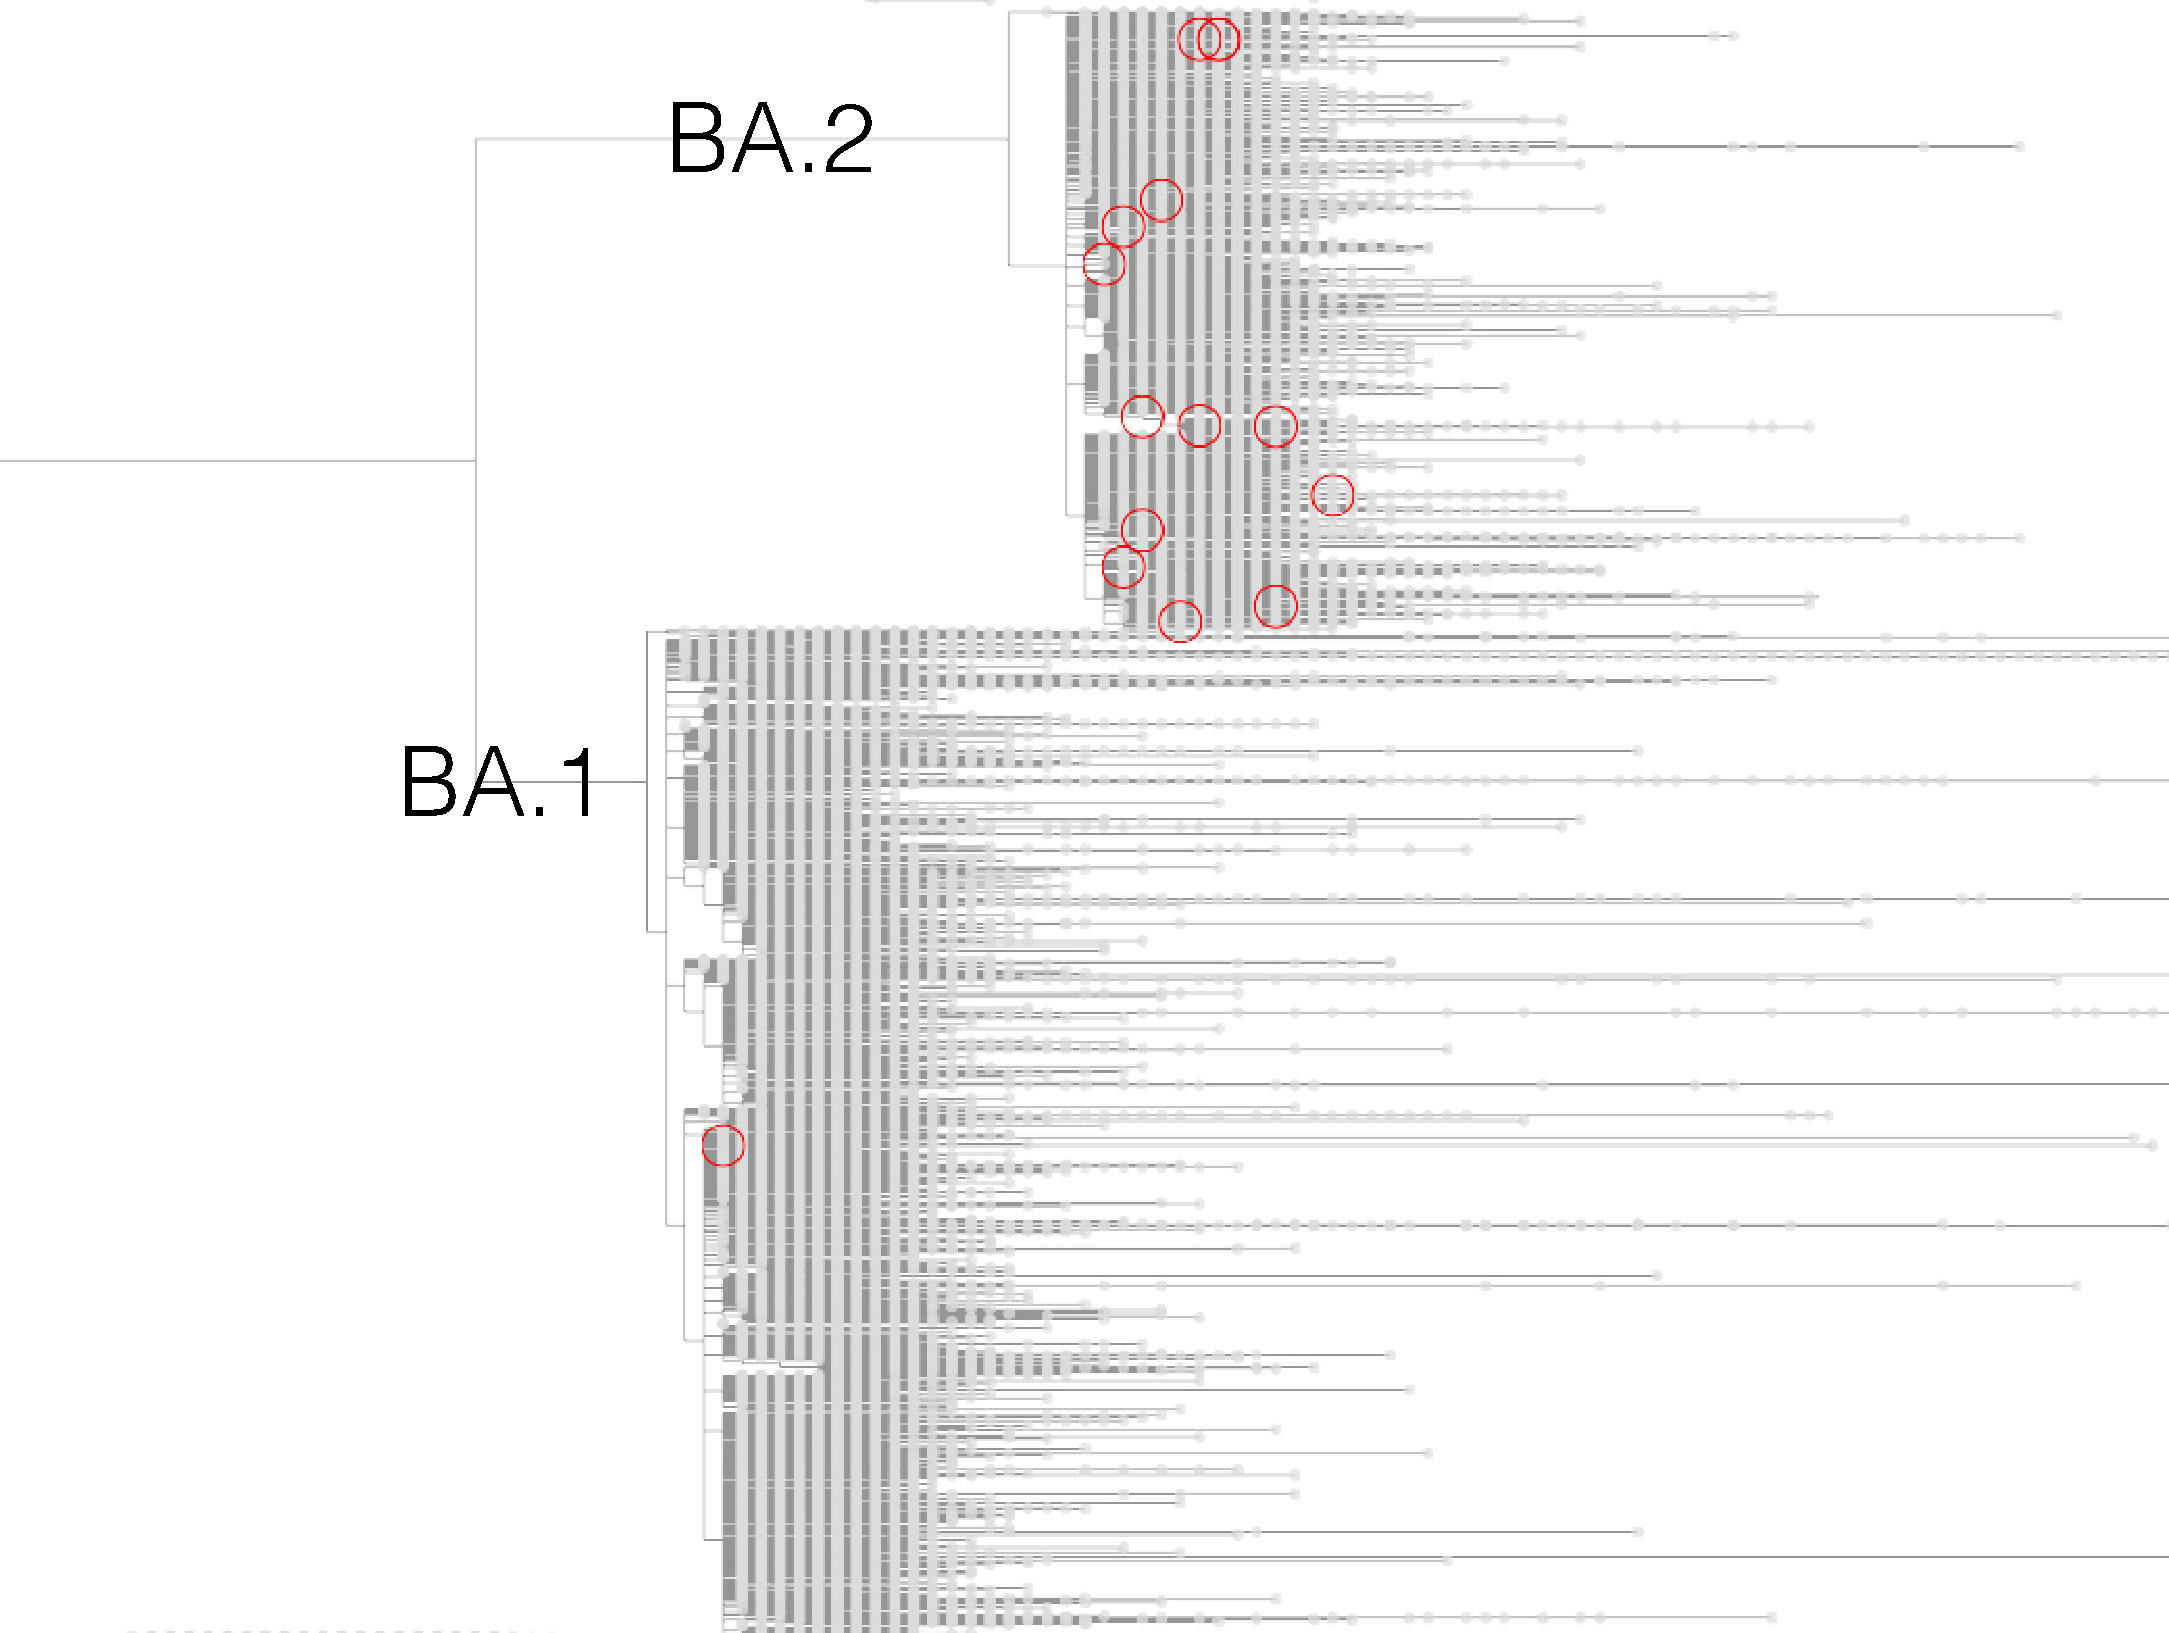
\includegraphics[width=\linewidth]{Figures/452.pdf}
\end{center}
\caption{Looking for recurrent mutations in SARS-CoV-2 with Taxonium. Here we have zoomed in on Omicron, with 1,184,788 sequences until mid-May 2022, and are circling nodes featuring a mutation at position S:452 which have more than 20 descendants. These appear to be much more common on the BA.2 genetic background. Labels have been added to the screenshot for clarity in this static format.}
\label{fig:452}
\end{figure}


The Taxonium web client can be used entirely client-side, without any interaction with a server, or it can be used in a server-backed mode, with a server providing the tree with data on demand, and the client visualising it. The server-backed mode is more efficient, as it does not require all data to be sent to the client, and the computationally expensive operations can be performed on a more powerful machine, but the client-side mode has the advantage that it can be used with custom data, and especially for data that may be sensitive and not suitable for uploading to a server. When used in client-side mode, these more expensive computational operations take place in a web worker, which ensures the main interface remains responsive.


\subsection*{The Taxonium Backend}

The Taxonium backend is implemented in NodeJS using Express, which means that much of the same code can be used in the client when it is running in full client-side mode. We have made substantial efforts to make the backend as efficient as possible. Nodes are stored sorted on their y-coordinates, permitting a binary search to rapidly find the indices of nodes that are within a given range of y-coordinates, corresponding to the region on which the user has zoomed.

\subsection*{Taxoniumtools}

We provide a simple Python application, taxoniumtools, which allows the user to generate a tree in Taxonium format from an Usher MAT.

Taxoniumtools [insert]


\subsection*{Cov2Tree}

We used Taxonium to build the Cov2Tree web application, which allows users to explore the global diversity of SARS-CoV-2 (Figure 2). Cov2Tree uses the UShER tree built by \cite{regular_updated}, which contains xx million sequences. It is the largest tree that has been made available to date. Cov2Tree is available at \url{http://Cov2Tree.org}. We provide a time tree inferred by Chronumental. We also provide the date placements inferred by Chronumental at [xxx] which can allow the identification of sequences with metadata errors \cite{chronumental}.

We run a server that supports the Cov2Tree application, meaning that the user needs only to download the data from the region of the tree on which they have zoomed in. This is particularly important to empower analysis in lower bandwidth settings. Users can colour the tree by pangolin lineage, by sample country, or by genotype.

In the case of the SARS-CoV-2 dataset, the server backend requires about 5 GB of RAM.




\begin{figure}
\begin{center}
\includegraphics[width=\linewidth]{figures/cov2tree_heatmap.png}
\end{center}
\caption{
A screenshot of the Cov2Tree application. The global tree is shown in the left hand panel, and the user has zoomed in on a region to the right of the global tree. The heatmap shows the sample dates and locations of the sequences in this region, and the legend shows how these are encoded in colour.
}
\label{fig:cov2tree}
\end{figure}


\section*{Discussion}\label{s:discussion}

In this paper we have introduced Taxonium, a web-based tool for browsing very large trees, including those annotated with mutations at internal nodes. Taxonium is open-source and freely available for use in any context. It is highly configurable, and can be used with any large tree. We have used Taxonium to build the Cov2Tree application, which allows users to explore the global diversity of SARS-CoV-2.

Taxonium is the first tool for tree exploration that scales to tens of millions of nodes. 



\section*{Methods}\label{s:methods}

\subsection*{Molecular biology}

\subsection*{Cell biology}



\section*{Bibliography}
\bibliographystyle{bxv_abbrvnat}
\bibliography{refs.bib}